\documentclass[11pt]{report}
\usepackage[spanish]{babel}
\usepackage[utf8]{inputenc}
\usepackage{Sweave}
\usepackage{graphicx}
\usepackage{hyperref}
\usepackage{anysize} 
\marginsize{1.78cm}{1.65cm}{1.78cm}{1.78cm} 

\title{\Huge Universidad Nacional de Loja \\ 
Área de la Energía las Industrias y los Recursos Naturales no Renovables \\
Ingeniería en Sistemas \\}

\author{
\includegraphics[width=5cm, height=5cm]{unl.jpg} \\\\\\\\
Antonio Aguilar Soto \\ waaguilars@unl.edu.ec \\\\
ECINF7224}\\\\

\begin{document}
\Sconcordance{concordance:L1_T1_1900481878.tex:L1_T1_1900481878.Rnw:%
1 42 1 1 5 4 0 1 5 1 2 2 1 1 5 4 0 1 1 4 0 1 2 2 1 1 5 4 0 1 1 3 0 1 1 %
4 0 1 2 2 1 1 5 1 2 3 1}

\maketitle

\begin{center}\textbf{ROCK DATASET}\end{center}
\textbf{Descripción}

El (aproximadamente) calificación trimestral aprobación para el Presidente de los Estados Unidos a partir del primer trimestre de 1945 hasta el último trimestre de 1.974.\\
\textbf{Uso:}
presidents
\\
\textbf{Formato}

Una serie de tiempo de 120 valores.
\textbf{Detalles}

Los datos son en realidad una versión amañadas de los índices de aprobación. Ver el libro de McNeil para más detalles.
\\
\textbf{Fuente}
La Organización Gallup.
\\
\textbf{Referencia}
McNeil, DR (1977) Análisis de Datos Interactivo. Nueva York: Wiley.
\\\\
\textbf{Determinar la estadística, cuando presidents son mayores a 1960.}

\begin{Schunk}
\begin{Soutput}
   Min. 1st Qu.  Median    Mean 3rd Qu.    Max.    NA's 
  24.00   46.00   58.00   56.07   68.75   83.00       2 
\end{Soutput}
\end{Schunk}
\\\\\\
\textbf{Determinar la estadística, cuando Qtr4 menores a 70 y mayores a 50, Cuál es el 3erQ?}

\begin{Schunk}
\begin{Soutput}
   Mode   FALSE    TRUE    NA's 
logical      15      13       2 
\end{Soutput}
\begin{Soutput}
75% 
 63 
\end{Soutput}
\end{Schunk}
\\\\\\
\textbf{ Determinar la estadística, cuando Qtr3 y Qtr4 están asignación (NA)}

\begin{Schunk}
\begin{Soutput}
   Min. 1st Qu.  Median    Mean 3rd Qu.    Max.    NA's 
  24.00   47.00   61.00   57.22   68.00   82.00       3 
\end{Soutput}
\begin{Soutput}
   Min. 1st Qu.  Median    Mean 3rd Qu.    Max.    NA's 
  23.00   44.00   55.50   53.07   63.00   78.00       2 
\end{Soutput}
\begin{Soutput}
   Min. 1st Qu.  Median    Mean 3rd Qu.    Max.    NA's 
   48.0    92.5   118.0   111.1   133.0   157.0       3 
\end{Soutput}
\end{Schunk}
\\\\\\
\textbf{Graficar Qtr1 Vs Qtr2, cuando Qtr2 no tiene asignación.}

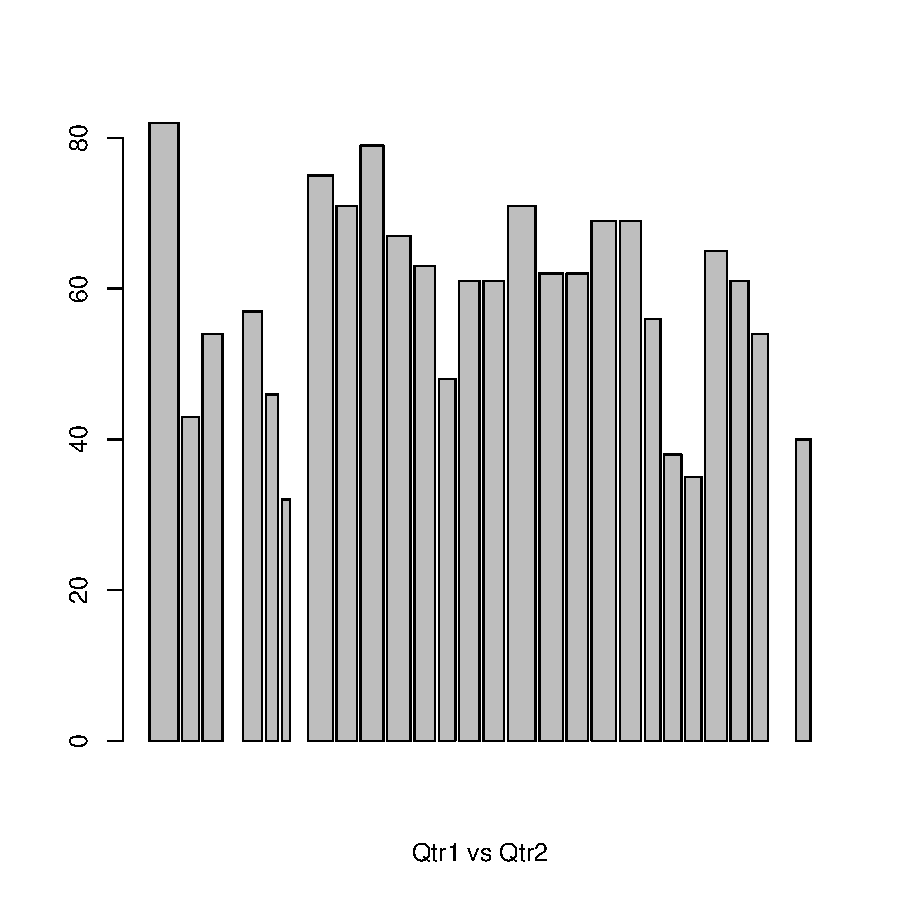
\includegraphics{L1_T1_1900481878-004}
\\\\\\


\includegraphics[width=3cm, height=2cm]{licencia.png}
\end{document}}
